

\section{Dynamics}

\subsection{Newton's laws}
\begin{definition}
    {Newton's first law}
    An object will remain at rest or in uniform motion unless acted upon by a force.
\end{definition}

\begin{definition}
    {Newton's second law}
    The acceleration of an object is directly proportional to the net force acting on it, and inversely proportional to its mass.
    \[\sum F=ma\]
\end{definition}

\begin{definition}
    {Newton's third law}
    For every action, there is an equal and opposite reaction. This gives rises to forces like friction, normal and tension forces.
\end{definition}

\begin{knBox}
    {Friction}
    Friction is a force that opposes the motion of an object. It is given by:
    \[F_f=\mu N\]
    Where $\mu$ is the coefficient of friction and $N$ is the normal force experienced by the object.
\end{knBox}

\begin{knBox}
    {Conservative force}
    Conservative forces are forces that do not depend on the path taken by an object. They also have no lost in energy. They include:
    \begin{enumerate}
        \item Gravitational force
        \item Elastic force
        \item Electric force
    \end{enumerate}
\end{knBox}

\begin{knBox}
    {Inertia force}
    Inertia force is the preceived force from the perspective of an accelerating object.
    \tcblower
    For a person in an elevator accelerating upwards at $a$, the inertia force is $ma$ downwards.
\end{knBox}

\subsection{Motion}
\begin{theorem}
    {Motion equations}
    The following are the equations of motion:
    \begin{itemize}
        \item \textbf{Average velocity: }$v=\frac{ds_t}{dt}$
        \item \textbf{Average acceleration: }$a=\frac{dv_t}{dt}$
        \item $s=ut+\frac{1}{2}at^2$
        \item $v=u+at$
        \item $v^2=u^2+2as$
        \item $s=\frac{(v+u)t}{2}$
    \end{itemize}
    Where $v$ is the final velocity, $u$ is the initial velocity, $a$ is the acceleration, $t$ is the time, and $s$ is the displacement.
\end{theorem}

\begin{theorem}
    {Circular  motion}
    The following are the equations of motion for circular motion:
    \begin{itemize}
        \item $\omega = \frac{\Delta\theta}{\Delta t}=\frac{2\pi r}{t} = \frac{v_t}{r}$
        \item $v_t = r\omega$
        \item $a_c = r\omega^2 = \frac{v_t^2}{r}$
        \item $a_t = r a_c$
        \item $F_c = \frac{mv_t^2}{r} = ma_c$
        \item \textbf{Total acceleration: }$a_{to} = \sqrt{a_t^2+a_c^2}$
        \item \textbf{Accelerating cylinder/disk: }$F = \frac12mra,\ Fr=Ia_c$
              $I_{disk}=\frac12mr^2$
    \end{itemize}
    \tcblower
    $\omega$ is the angular velocity, which describes change in angle over time\\
    $\{v_t,\ a_t\}$ is the tangential velocity and acceleration, which is tangential to any point on the radius\\
    $\{a_c,\ F_c\}$ is the centripetal acceleration and force, which are perpendicular to tangential quantities. They act on the object, hence they be seen as normal forces.\\
    $a_{to}$ is the total acceleration, which is the resultant of $a_t$ and $a_c$
\end{theorem}

\begin{knBox}
    {Direction of angular velocity}
    The direction of the angular velocity is given by the right-hand rule. If the fingers of the right hand curl in the direction of rotation, the thumb points in the direction of the angular velocity.
\end{knBox}

\begin{knBox}
    {Instantaneous center of zero velocity}
    The instantaneous center of zero velocity is the point on a rotating object that has zero velocity. The velocity is perpendicular to the radius (edge) at that point.
    \begin{center}
        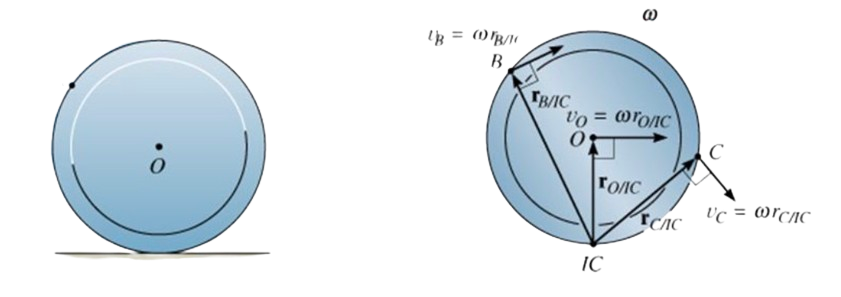
\includegraphics[width=0.5\textwidth]{./img/ic.png}
    \end{center}
    The velocity at any point is given by:
    \[v=\omega d\]
    Where $d$ is the distance from the IC.
\end{knBox}

\subsection{Momentum and impulse}

\begin{definition}
    {Momentum and conservation of momentum}
    Momentum is the product of an object's mass and velocity. It is a vector quantity.
    \[p=mv\]
    The principle of conservation of momentum states that the total momentum of a system remains constant if no external forces act on it.
    \[F_{ext}=0\ ?\ p=\text{const}\]
    The angular momentum about a point $O$ is given by:
    \[H_O=Iw=mv_i\times r\]
\end{definition}

\begin{theorem}
    {Coefficient of restitution}
    The coefficient of restitution is a measure of how much kinetic energy is conserved in a collision. It is given by:
    \[e=|\frac{v_{2}-v_{1}}{u_{1}-u_{2}}|\]
    Where $v_{1}$ and $v_{2}$ are the final velocities, and $u_{1}$ and $u_{2}$ are the initial velocities.
    \begin{itemize}
        \item $e=1$ is a perfectly elastic collision
        \item $e=0$ is a perfectly inelastic collision
        \item $0<e<1$ is a (partially) elastic collision
    \end{itemize}
\end{theorem}

\begin{definition}
    {Impulse (impact)}
    Impulse is the change in momentum of an object. It is given by:
    \[\Delta p=F\Delta t\]
\end{definition}

\subsection{Vibrations}

\subsubsection{Simple harmonic motion}
\begin{theorem}
    {Simple Harmonic Motion equations}
    The following are the equations of motion for simple harmonic motion:
    \begin{itemize}
        \item $x=A\sin(wt+\phi)$
        \item $f=\frac{1}{T}=\frac{w}{2\pi}$
        \item $T_{vertical} = 2\pi\sqrt{\frac{m}{k}}$
        \item $T_{swing} = 2\pi\sqrt{\frac{l}{g}}$
    \end{itemize}
    Where $A$ is the amplitude. $\phi$ represents the angle of which the motion starts. ($\Delta\phi$ for $x$ from $x=0$ to $x:t=0$ )
\end{theorem}

\begin{definition}
    {Natural frequency}
    The natural frequency of a spring mass system is the frequency at which the system oscillates when displaced from equilibrium.
    \[w_0=\sqrt{\frac{k}{m}}\]
    Where $f$ is the frequency, $k$ is the spring constant, and $m$ is the mass.
\end{definition}

\subsubsection{Spring mass system}

\begin{definition}
    {Hooke's law}
    Hooke's law states that the force required to extend or compress a spring is directly proportional to the extension or compression.
    \[F=-kx\]
    Where $F$ is the force, $k$ is the spring constant, and $x$ is the extension or compression.
\end{definition}

\begin{definition}
    {Damping \& damping coefficient}
    Damping is the process of reducing the amplitude of an oscillation. It is given by:
    \[F_d=-cv\]
    Where $F_d$ is the damping force, $c$ is the \textbf{damping coefficient}, and $v$ is the velocity.
\end{definition}

\begin{theorem}
    {Critical damping}
    Critical damping is the minimum amount of damping required to prevent oscillation. It is given by:
    \[c_{crit}=2\sqrt{mk}\]
    The following gives the cases of damping:
    \begin{itemize}
        \item \textbf{Underdamping: }$c<c_{crit}$
        \item \textbf{Overdamping: }$c>c_{crit}$
        \item \textbf{Critical damping: }$c=c_{crit}$
    \end{itemize}
    Critical damping gives the fastest return to equilibrium.
\end{theorem}

\subsection{Energy, work and power}

\begin{definition}
    {Work}
    Work done is the energy required to move an object. It is given by:
    \[W=Fd\]
\end{definition}

\begin{theorem}
    {Energy}
    The following are the types of energy:
    \begin{itemize}
        \item \textbf{Kinetic: }$E_k=\frac{1}{2}mv^2$
        \item \textbf{Gravitational potential: }$E_{GP}=mgh$
        \item \textbf{Elastic potential: }$E_{EP}=\frac{1}{2}kx^2$
        \item \textbf{Friction: } $E_{f}=F_f\times d=\mu Nd$
        \item \textbf{Rotational: } $E_{r}=\frac{1}{2}Iw^2=\frac14mv_t^2$
    \end{itemize}
    The energy of a spring-mass system is given by:
    \[E=E_k+E_{EP}\]
\end{theorem}

\begin{theorem}
    {Conversation of energy}
    The principle of conservation of energy states that the total energy of a system remains constant if no external forces act on it.
    \[F_{ext}=0\ ?\ E=\text{const}\]
    This means in a system, energy is converted from one form to another. Use this fact to solve for unknowns.
\end{theorem}

\begin{definition}
    {Power}
    Power is the rate at which work is done. It is given by:
    \[P=\frac{W}{t}\]
\end{definition}

\begin{theorem}
    {Power and acceleration}
    The power required to accelerate an object is given by:
    \[P=Fv\]
    Where $F$ is the force, and $v$ is the velocity.
\end{theorem}